\documentclass[a4paper,11pt,oneside,onecolumn]{article}
\usepackage[utf8]{inputenc}
\usepackage{cmap}
\usepackage[T1]{fontenc}
\usepackage{beton}
\usepackage{eulervm}
\renewcommand{\sfdefault}{\rmdefault}
\usepackage[pdftex,colorlinks,citecolor=black,filecolor=black,linkcolor=black,urlcolor=black]{hyperref}
\usepackage{tikz}
\usetikzlibrary{positioning,arrows,automata,decorations.pathreplacing,decorations.text,decorations.markings,arrows,shapes,calc,fit}
\usepackage{caption}
\usepackage{subcaption}
\usepackage{multirow}
\usepackage{hhline}
\usepackage{graphicx}
\usepackage{amsmath}
\usepackage[noend]{algpseudocode}

\newcommand{\comment}[1]{%
  \text{\phantom{(#1)}} \tag{#1}
}

\title{Homework 4}
\author{Mitar Milutinovic (24090156)\thanks{Worked together with Shiry Ginosar, Valkyrie Savage, Orianna DeMasi.}}

\renewcommand\thesection{\arabic{section}.}
\renewcommand\thesubsection{\thesection (\alph{subsection})}

\begin{document}

\maketitle

\section{}

\subsection{}

An example of a non-bipartite graph which have a non-integer optimum solution.

\begin{center}
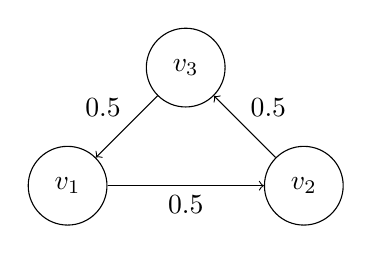
\begin{tikzpicture}

\node[draw,circle,minimum size=1cm] (a) at (0,0) {$v_1$};
\node[draw,circle,minimum size=1cm] (b) at (3,0) {$v_2$};
\node[draw,circle,minimum size=1cm] (c) at (1.5,1.5) {$v_3$};
\draw[->] (a) -- node[below] {$0.5$} (b);
\draw[->] (b) -- node[above,xshift=0.3cm] {$0.5$} (c);
\draw[->] (c) -- node[above,xshift=-0.3cm] {$0.5$} (a);

\end{tikzpicture}
\end{center}

All edges have weight 1, the optimal solution for linear program is 1.5.

\subsection{}

Linear program with a set of constraints corresponding to Edmonds' condition.

\begin{align*}
\max \sum_e w_e x_e &  \\
\forall v \in V: \sum_{e=(u,v)} x_e & \le 1 \\
\forall S \subseteq V, |S| \textrm{ is odd}: \sum_{e=(u,v) \in (S \times (V \setminus S))} x_e & \ge 1 \\
x_e & \ge 0 \\
\end{align*}

\subsection{}

For the dual, we introduce new variables for nontrivial constraints from the primal. For the first constraint, for each
vertex $v$ constraint, we introduce variable $y_v$. For the second constraint, for each $S$ constraint, we introduce variable
$y_S$. The resulting linear program is then:

\begin{align*}
\min \sum_v y_v + \sum_{S \subseteq V, |S| \textrm{ is odd}} y_S & \\
\forall e = (u,v) \in E: y_u + y_v - \sum_{S \subseteq V, |S| \textrm{ is odd}, u \in S, v \in (V \setminus S)} y_S & \ge w(e) \\
y_v & \ge 0 \\
y_S & \ge 0 \\
\end{align*}

Interpretation is similar to the interpretation for the algorithm to solve the maximum weight matching and minimum vertex cover
for bipartite graphs. Additionally, here we have odd cuts which put additional better limit on new edges we are using in the
alternating paths part of the algorithm, guiding us in this generalized algorithm.

To be able to use this on the example graph from (a), we have to have even number of vertices. So we add a dummy vertex $v_d$.

\begin{center}
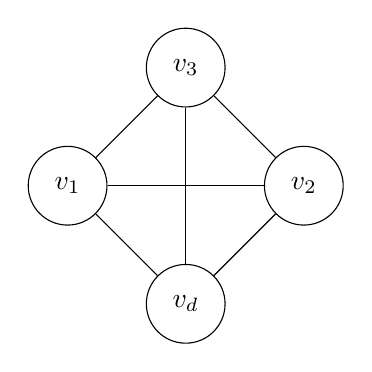
\begin{tikzpicture}

\node[draw,circle,minimum size=1cm] (a) at (0,0) {$v_1$};
\node[draw,circle,minimum size=1cm] (b) at (3,0) {$v_2$};
\node[draw,circle,minimum size=1cm] (c) at (1.5,1.5) {$v_3$};
\node[draw,circle,minimum size=1cm] (d) at (1.5,-1.5) {$v_d$};
\draw[-] (a) -- (b);
\draw[-] (b) -- (c);
\draw[-] (c) -- (a);
\draw[-] (d) -- (a);
\draw[-] (d) -- (b);
\draw[-] (d) -- (c);

\end{tikzpicture}
\end{center}

Solving the dual for this extended example gives us a feasible solution of value 1. Based on weak duality, we know that this
value is an upper bound for the primal optimal solution. This means primal solution cannot be larger than 1 and cannot
achieve 1.5 which we found as an optimal fractional value. So, no integer solution can have the value 1.5.

\section{}

\subsection{}

We have two convex bodies $A$ and $B$ which do not intersect. We choose point $a \in A$ so that it is the closest point
to $B$. Similarly, we choose
point $b \in B$ so that it is the closest point to $A$. Using normal $(a,b)$ we construct a hyperplane between $A$ and $B$.
If the hyperplane intersects $A$ or $B$ in some point, then $a$ or $b$, respectively, could not be the closest points.
Alternatively, the bodies are not convex or they are intersecting. In any case, assumptions do not hold.

\subsection{}

Farkas B says that true is exactly one of:
\begin{enumerate}
\item $\exists x: Ax \le b$, or
\item $\exists y: y^TA = 0, y^Tb < 0 , y \ge 0$
\end{enumerate}

Both 1.~and 2.~cannot be true at the same time, because it brings us to a contradiction:

\begin{align*}
Ax & \le b \\
y^TAx & \le y^Tb \\
y^TAx & \le y^Tb < 0 \\
0 = y^TAx & \le y^Tb < 0 \\
0 & < 0 \\
\end{align*}

If 1.~does not hold, then 2.~must hold. Let's assume 1.~does not hold, so:

\begin{align*}
Ax & > b \\
b - Ax & < 0 \\
\end{align*}

We know that spaces $b - Ax < 0$ and $x \ge 0$ are convex and nonintersecting, so there exists a separating hyperplane
between them. There exists $y$ such that $y^T(b - Ax) < 0$ and $y^Tx \ge 0$. Because $y^Tx \ge 0$ holds for $x \ge 0$,
$y^T \ge 0$ must hold and thus $y \ge 0$ holds as well.

\begin{align*}
y^T(b - Ax) & < 0 \\
y^Tb - y^TAx & < 0 \\
\end{align*}

By chosing $x=0$, we get $y^Tb < 0$.

If we assume $y^TA = 0$ does not hold, then $y^TA \ne 0$. But this brings us to a contradiction $ y^Tb - y^TAx \ge 0 $
for any $x$ such that:

\begin{align*}
y^Tb - y^TAx & \ge 0 \\
y^Tb & \ge y^TAx \\
\frac{y^Tb}{y^TA} & \ge x \\
\frac{b}{A} & \ge x \\
\end{align*}

This proves that Farkas B holds.

\section{}

\subsection{}

We assume $C' > C$, otherwise it is trivial. With $F$ and $C$ we denote the optimal facility and connection cost respectively.
Given solution has connection cost $C'$. Because $C' > C$ we know that there is a non-empty set of facilities which are not
yet open but are open in the optimal solution. These facilities have facility costs $f_i$ and connection costs $c_i$.
We know that $ 0 < \sum f_i \le F $, trivially, and $ \sum c_i \ge C' - C $, because the difference between $C'$ and $C$ is
by definition that which we cover by opening $c_i$ facilities. Combining this two inequalities:

$$
\frac{\sum c_i}{\sum f_i} \ge \frac{C' - C}{F}
$$

There exist a facility $k$, $c_k = \Delta$, $f_k = f$, so that:

$$
\frac{\Delta}{f} = \frac{c_k}{f_k} \ge \frac{\sum c_i}{\sum f_i} \ge \frac{C' - C}{F}
$$

If we assume that such facility does not exist, we get a contradiction:

\begin{align*}
\frac{c_k}{f_k} & < \frac{\sum c_i}{\sum f_i} = X \\
c_k & < X f_k \\
\sum c_k & < X \sum f_k \\
\sum c_i & < X \sum f_i \\
X = \frac{\sum c_i}{\sum f_i} & < X \frac{\sum f_i}{\sum f_i} = X \\
X & < X \\
\end{align*}

\subsection{}

Based on a known facility location solution with expected total cost of $2F + 3C$ we can repeat the step from question (a) while it
is reasonable to do so, ie., while gain from decreasing connection costs is larger than costs of opening a new facilty,
$c_k > f_k$. We can write this condition also as:

\begin{align*}
1 > \frac{c_k}{f_k} & \ge \frac{C' - C}{F} \\
F & > C' - C \\
C' & < F + C \\
\end{align*}

From this we can conclude, that expected final connection cost using step from question (a) is $F + C$. But as we were improving
connection cost, we were increasing facility cost. Starting at $F$ at each step we open a new facility with cost
$f_k \le \frac{c_k F}{C' - C}$. Total facility cost is thus:

\begin{align*}
F + \sum f_k & \le F + \sum \frac{c_k F}{C' - C} \\
& = F\left(1 + \sum \frac{c_k}{C' - C}\right) \\
& = F\left(1 + \int\limits_{F+C}^{2F + 3C} \frac{\mathrm{d}C'}{C' - C}\right) \\
& = F\left(\left. 1 + \ln(C' - C)\right|_{F+C}^{2F + 3C} \right) \\
& = F\left( 1 + \ln(2F + 2C) - \ln(F) \right) \\
& = F\left( 1 + \ln\frac{2F + 2C}{F} \right) \\
\end{align*}

Commutative expected total connection and facility cost is therefore $F + C + F\left( 1 + \ln\frac{2F + 2C}{F} \right)$.

\subsection{}

We open each facility $i$ with probability $y_i$. In a rare case that no facilities have been opened, we open one with
lowest facility cost, $f_{\min}$. After we have determined which facilities are open, we route each client $i$ to closest open
facility $k$ when $x_{ki} > 0$, or any open facility otherwise, at connection cost $3$.

Expected facility cost of the algorithm is sum of two cases -- when no facility opened and when at least one facility opened:

\begin{align*}
& P(n=0) f_{\min} + P(n>0)\sum y_i f_i \\
& = \prod(1 - y_i) f_{\min} + \left(1 - \prod(1 - y_i)\right) F \\
& \le F + \prod(1 - y_i) f_{\min} \\
\end{align*}

Similarly, expected connection cost is sum of two cases -- that client $i$ has no facility $k$ open with $x_{ki} > 0$, or he has. The latter
probability is:

\begin{align*}
& 1 - \prod_{x_{ki} > 0} (1 - y_k) \\
& \ge 1 - \prod_{x_{ki} > 0} (1 - x_{ki}) \\
& \ge 1 - \left( 1 - \frac{1}{n} \right)^n \\
& \ge 1 - \frac{1}{e} \\
\end{align*}

It follows that the former probability is $\frac{1}{e}$, at connection cost $3$. Expected connection cost is thus upper bounded by the sum:

\begin{align*}
& \sum \left( \left( 1 - \frac{1}{e} \right) C(i) + \frac{1}{e} 3 \right) \\
& \le \left( 1 - \frac{1}{e} \right) C + \frac{3}{e} N_c \\
& \le \left( 1 - \frac{1}{e} \right) C + \frac{3}{e} C \\
& = \left( 1 + \frac{2}{e} \right) C \\
\end{align*}

\section{}

From knowing second moments from which we can compute the size of join by:

$$
\sum f_r(a)f_s(a) = \frac{1}{2} \sum \left( (f_r(a) + f_s(a))^2 - f_r(a)^2 - f_s(a)^2 \right)
$$

$\sum (f_r(a) + f_s(a))^2$, $\sum f_r(a)^2$, and $\sum f_s(a)^2$ can be computer using known streaming second moments algorithm.

Second moment error for the streaming algorithm can be defined as $1 \pm \epsilon$. Cumulative error is so:

\begin{align*}
& \frac{1}{2} \left( (f_r(a) + f_s(a))^2 (1 \pm \epsilon) - f_r(a)^2 (1 \pm \epsilon) - f_s(a)^2 (1 \pm \epsilon) \right) \\
& = \frac{1}{2} \left( \left( f_r(a)^2 + 2 f_r(a) f_s(a) + f_s(a)^2 \right) (1 \pm \epsilon) - f_r(a)^2 (1 \pm \epsilon) - f_s(a)^2 (1 \pm \epsilon) \right) \\
& = \frac{1}{2} \left( 2 f_r(a) f_s(a) (1 \pm \epsilon) \pm f_r(a)^2 2 \epsilon \pm f_s(a)^2 2 \epsilon \right) \\
& = f_r(a) f_s(a) (1 \pm \epsilon) \pm f_r(a)^2 \epsilon \pm f_s(a)^2 \epsilon \\
& = f_r(a) f_s(a) \pm \epsilon ( f_r(a) f_s(a) + f_r(a)^2 + f_s(a)^2 ) \\
\end{align*}

\section{}

We designed a voting schema which allows a group of people to better decide on a common opinion about an issue. Currently,
the most used approach is to simply count number of votes against and for, while not taking into account people who do
not cast a vote. Our approach is to have each person define delegates whose votes will be counted when he/she does not
vote him/herself. In this way we get a social network, a trust network, between users which can be
used to transitively compute missing votes. We believe such a result better represents the will of the group.

In the course of the project, we want to compare it with some other similar voting schemas with delegation. We want to visualize
our approach and possibly find a way to visualize differences to other schemas. We will analyze the algorithm for computing the
results according to our voting schema.

On the project I will be working with Valkyrie Savage.

\end{document}
